%% 25 minutes + 5 minutes Q&A

\documentclass[pdftex,aspectratio=169]{beamer}

\usepackage[utf8]{inputenc}
\usepackage{theme/beamerthemeUFR}
\usepackage{amsmath}
\usepackage{amssymb}
\usepackage{mathtools}
\usepackage{bbold}
\usepackage{yfonts}
\usepackage{stmaryrd}
\usepackage{mathpartir}
\usepackage{booktabs}
\usepackage{array}
\usepackage{tikz}
\usetikzlibrary{arrows.meta,positioning,calc}
\usepackage{appendixnumberbeamer}

% Agda's LaTeX backend and the code fragments extracted by runagdatex.
\usepackage{latex/agda}
\providecommand{\lambdabar}{{\mkern0.75mu\mathchar '26\mkern-9.75mu\lambda}}
% Local copy of https://github.com/Mari-W/Agdasubst (tex/esop27, commit f8419ed, Marius Weidner).
% Maps the Unicode characters of the Agda code to LaTeX symbols for pdflatex.
\usepackage{dsfont}
\usepackage{newunicodechar}
\newunicodechar{λ}{\ensuremath{\mathnormal\lambda}}
\newunicodechar{σ}{\ensuremath{\mathnormal\sigma}}
\newunicodechar{τ}{\ensuremath{\mathnormal\tau}}
\newunicodechar{π}{\ensuremath{\mathnormal\pi}}
\newunicodechar{ℕ}{\ensuremath{\mathbb{N}}}
\newunicodechar{∷}{\ensuremath{::}}
\newunicodechar{≡}{\ensuremath{\equiv}}
\newunicodechar{≅}{\ensuremath{\cong}}
\newunicodechar{∀}{\ensuremath{\forall}}
\newunicodechar{ᴸ}{\ensuremath{^L}}
\newunicodechar{ᴿ}{\ensuremath{^R}}
\newunicodechar{ʳ}{\ensuremath{^r}}
\newunicodechar{ᶻ}{\ensuremath{^Z}}
\newunicodechar{ₗ}{\ensuremath{_l}}
\newunicodechar{ⱽ}{\ensuremath{^V}}
\newunicodechar{⟧}{\ensuremath{\rrbracket}}
\newunicodechar{⟦}{\ensuremath{\llbracket}}
\newunicodechar{⊤}{\ensuremath{\top}}
\newunicodechar{⊥}{\ensuremath{\bot}}
\newunicodechar{₁}{\ensuremath{_1}}
\newunicodechar{₂}{\ensuremath{_2}}
\newunicodechar{₃}{\ensuremath{_3}}
\newunicodechar{₄}{\ensuremath{_4}}
\newunicodechar{₅}{\ensuremath{_5}}
\newunicodechar{₆}{\ensuremath{_6}}
\newunicodechar{₇}{\ensuremath{_7}}
\newunicodechar{₈}{\ensuremath{_8}}
\newunicodechar{₉}{\ensuremath{_9}}
\newunicodechar{∈}{\ensuremath{\in}}
\newunicodechar{₀}{\ensuremath{_0}}
\newunicodechar{′}{\ensuremath{'}}
\newunicodechar{ˢ}{\ensuremath{^S}}
\newunicodechar{ᴬ}{\ensuremath{^A}}
\newunicodechar{∘}{\ensuremath{\circ}}
\newunicodechar{𝟙}{\ensuremath{\mathds{1}}}  
\newunicodechar{𝟘}{\ensuremath{\mathds{O}}}
% \newunicodechar{𝟙}{\ensuremath{\mathbb{I}}}  
% \newunicodechar{𝟘}{\ensuremath{\mathbb{O}}}
\newunicodechar{ᴾ}{\ensuremath{^P}}
\newunicodechar{ᵀ}{\ensuremath{^T}}
\newunicodechar{⊎}{\ensuremath{\uplus}}
\newunicodechar{ι}{\ensuremath{\iota}}
\newunicodechar{⇐}{\ensuremath{\Leftarrow}}
\newunicodechar{⇒}{\ensuremath{\Rightarrow}}
\newunicodechar{➙}{\ensuremath{\to^P}}
\newunicodechar{Δ}{\ensuremath{\Delta}}
\newunicodechar{∅}{\ensuremath{\emptyset}}
\newunicodechar{⁺}{\ensuremath{^+}}
\newunicodechar{𝕏}{\ensuremath{\mathbb{X}}}
%\newunicodechar{·}{\ensuremath{\cdot}} %seems to be defined already!
\newunicodechar{∙}{\ensuremath{\cdot}}
\newunicodechar{⁇}{\ensuremath{?}}
\newunicodechar{‼}{\ensuremath{!}}
\newunicodechar{⊕}{\ensuremath{\oplus}}
\newunicodechar{ℤ}{\ensuremath{\mathbb{Z}}}
\newunicodechar{μ}{\ensuremath{\mu}}
\newunicodechar{∃}{\ensuremath{\exists}}
\newunicodechar{；}{\ensuremath{\fatsemi}}
\newunicodechar{Σ}{\ensuremath{\Sigma}}
\newunicodechar{ᵢ}{\ensuremath{_i}}
\newunicodechar{≢}{\ensuremath{\nequiv}}
\newunicodechar{≟}{\ensuremath{\stackrel{{\tiny?}}{=}}}
\newunicodechar{≤}{\ensuremath{\le}}
\newunicodechar{ᵇ}{\ensuremath{^b}}
\newunicodechar{𝓣}{\ensuremath{\mathcal{T}}}
\newunicodechar{𝓔}{\ensuremath{\mathcal{E}}}
\newunicodechar{Γ}{\ensuremath{\Gamma}}
\newunicodechar{γ}{\ensuremath{\gamma}}
\newunicodechar{⊔}{\ensuremath{\sqcup}}
\newunicodechar{α}{\ensuremath{\alpha}}
\newunicodechar{η}{\ensuremath{\eta}}
\newunicodechar{ω}{\ensuremath{\omega}}
\newunicodechar{◁}{\ensuremath{\lhd}}
%PT: seems to be already defined
%\newcommand{\lambdabar}{{\mkern0.75mu\mathchar '26\mkern -9.75mu\lambda}}
\newunicodechar{ƛ}{\ensuremath{\lambdabar}}
\newunicodechar{Λ}{\ensuremath{\mathnormal\Lambda}}
\newunicodechar{ρ}{\ensuremath{\rho}}
\newunicodechar{𝓖}{\ensuremath{\mathcal{G}}}
\newunicodechar{ℓ}{\ensuremath{\ell}}
\newunicodechar{♯}{\ensuremath{\sharp}}
\newunicodechar{⇓}{\ensuremath{\Downarrow}}
\newunicodechar{𝓥}{\ensuremath{\mathcal{V}}}
\newunicodechar{∧}{\ensuremath{\wedge}}
\newunicodechar{ₛ}{\ensuremath{_s}}
\newunicodechar{χ}{\ensuremath{\chi}}
\newunicodechar{⊨}{\ensuremath{\models}}
\newunicodechar{⦂}{\ensuremath{\mathbf{:}}}
\newunicodechar{ς}{\ensuremath{\varsigma}}
\newunicodechar{𝓓}{\ensuremath{\mathcal{D}}}
\newunicodechar{∎}{\ensuremath{\square}}
\newunicodechar{■}{\ensuremath{\blacksquare}}
\newunicodechar{↠}{\ensuremath{\twoheadrightarrow}}
\newunicodechar{↪}{\ensuremath{\hookrightarrow}}
\newunicodechar{ⁱ}{\ensuremath{^i}}
\newunicodechar{Π}{\ensuremath{\Pi}}
\newunicodechar{∋}{\ensuremath{\ni}}
\newunicodechar{∍}{\ensuremath{\ni}}
\newunicodechar{‵}{\ensuremath{`}}
\newunicodechar{⨆}{\ensuremath{\bigsqcup}}
\newunicodechar{δ}{\ensuremath{\delta}}
\newunicodechar{κ}{\ensuremath{\kappa}}
\newunicodechar{⦃}{\ensuremath{\{\!|}}  % \lBrace from stix
\newunicodechar{⦄}{\ensuremath{|\!\}}}  % \rBrace from stix
\newunicodechar{⌊}{\ensuremath{\lfloor}}
\newunicodechar{⌋}{\ensuremath{\rfloor}}
\newunicodechar{𝟎}{\ensuremath{\mathbf{0}}}
\newunicodechar{𝟏}{\ensuremath{\mathbf{1}}}
\newunicodechar{𝟐}{\ensuremath{\mathbf{2}}}
\newunicodechar{β}{\ensuremath{\beta}}
\newunicodechar{≥}{\ensuremath{\geq}}
\newunicodechar{ₒ}{\ensuremath{_o}}
\newunicodechar{∊}{\ensuremath{\in}}
\newunicodechar{;}{\ensuremath{;}}
\newunicodechar{⋯}{\ensuremath{\mkern2mu \cdotp \mkern-2mu \cdotp \mkern-2mu \cdotp \mkern1mu }}
\newunicodechar{⊢}{\ensuremath{\vdash}}
\newunicodechar{∶}{\ensuremath{:}}
\newunicodechar{★}{\ensuremath{\star}}
\newunicodechar{ᴷ}{\ensuremath{^K}}
\newunicodechar{ϕ}{\ensuremath{\varphi}}
\newunicodechar{ᴮ}{\ensuremath{^B}}
\newunicodechar{＋}{}
\newunicodechar{ᵣ}{\ensuremath{_r}}
\newunicodechar{ₓ}{\ensuremath{_x}}
\newunicodechar{ₜ}{\ensuremath{_t}}
\newunicodechar{𝓡}{\ensuremath{\mathcal{R}}}
\newunicodechar{𝓢}{\ensuremath{\mathcal{S}}}
\newunicodechar{𝓚}{\ensuremath{\mathcal{K}}}
\newunicodechar{ᴹ}{\ensuremath{^M}}
\newunicodechar{ᵗ}{\ensuremath{^t}}
\newunicodechar{ξ}{\ensuremath{\xi}}
\newunicodechar{≐}{\ensuremath{\doteq}}
\newunicodechar{⸴}{\ensuremath{,}}
\newunicodechar{ᴱ}{\ensuremath{^E}}
\newunicodechar{⨟}{\ensuremath{\fatsemi}}
\newunicodechar{▷}{\ensuremath{\rhd}}
\newunicodechar{⟶}{\ensuremath{\longrightarrow}}
\newunicodechar{ᵏ}{\ensuremath{^k}}
\newunicodechar{∗}{\ensuremath{\ast}}
\newunicodechar{Φ}{\ensuremath{\Phi}}
\newunicodechar{∣}{\ensuremath{\mid}}
\newunicodechar{⇑}{\ensuremath{\Uparrow}}
\newunicodechar{ζ}{\ensuremath{\zeta}}
\newunicodechar{⊚}{\ensuremath{\odot}}
\newunicodechar{ᶜ}{\ensuremath{^c}}
\newunicodechar{⨾}{\ensuremath{\fatsemi}} % homonymous!
\newunicodechar{Ψ}{\ensuremath{\Psi}}
\newunicodechar{≠}{\ensuremath{\neq}}
\newunicodechar{⟪}{\ensuremath{\langle\!\langle}}
\newunicodechar{⟫}{\ensuremath{\rangle\!\rangle}}

\newunicodechar{●}{\ensuremath{\bullet}}
\newunicodechar{↑}{\ensuremath{\uparrow}}
\newunicodechar{→}{\ensuremath{\to}}
\input{agda-generated}

\setbeamertemplate{navigation symbols}{}
\setbeamertemplate{blocks}[rounded][shadow=true]
\everymath{\displaystyle}

\definecolor{sigmafill}{RGB}{229,236,248}
\definecolor{rorfill}{RGB}{226,242,233}
\definecolor{ewfill}{RGB}{252,236,232}
\definecolor{muted}{RGB}{90,96,104}

\newcommand{\refl}{\texttt{refl}}
\newcommand{\yes}{\textcolor{alu-green}{\checkmark}}
\newcommand{\no}{\textcolor{alu-red}{\(\times\)}}
\newcommand{\Blob}{\ensuremath{\bullet}}
\newcommand{\Wk}{\ensuremath{\mathord{\uparrow}}}
\newcommand{\Subst}[2]{#1\,[#2]}
\newcommand{\Ror}{\textsc{RoR}}
\newcommand{\source}[1]{\vfill{\scriptsize\color{muted}#1}}
\newcommand{\highlightbox}[2][alu-darkblue]{%
  \begin{beamercolorbox}[rounded=true,sep=.65em,wd=\linewidth]{block body}%
    \color{#1}#2
  \end{beamercolorbox}}

\tikzset{
  system/.style={draw,rounded corners=2pt,minimum height=1.15cm,
    align=center,font=\small,inner xsep=8pt},
  implication/.style={-{Stealth[length=2.5mm]},line width=1.0pt,alu-darkblue}
}

\title[All You Need Is \refl]{All You Need Is \refl{} --- Almost}
\subtitle{Return of the Renamings}
\author[Thiemann \& Weidner]{Peter Thiemann \quad Marius Weidner}
\institute[IIF]{Wadler70 @ Edinburgh}
\date{09 Sep 2026}
\titlegraphic{}

\begin{document}
{
\usebackgroundtemplate{%
  
\includegraphics[width=\paperwidth,height=\paperheight]{return-of-the-renamings.png}%
}
\begin{frame}[plain]
\end{frame}
}
\begin{frame}[plain,label=fp]
  \titlepage
\end{frame}

\section{The question}

\begin{frame}{Substitution in PL metatheory: a solved problem?}
  \begin{columns}[T,onlytextwidth]
    \begin{column}{.47\textwidth}
      \begin{block}<1->{On paper}
        \centering
        \vspace{.25em}
        \(M[x:=N]\)
        \vspace{.5em}

        \small ``capture-free substitution''\\
        ``Barendregt convention''
      \end{block}
    \end{column}
    \begin{column}{.47\textwidth}
      \begin{alertblock}<2->{In a proof assistant}
        \small
        representations (vectors, functions, \dots),\\ renamings,\\ composition lemmas,\\ \dots
      \end{alertblock}
    \end{column}
  \end{columns}

  \uncover<3->{%
    \vspace{1.0em}
    \begin{center}
      \Large What if substitution lemmas were
      \textbf{definitional}?
    \end{center}

    \vspace{.4em}
    \begin{center}
      \color{alu-darkblue}\Large proof = \refl
    \end{center}
  }
\end{frame}

\begin{frame}{Automated Proof}
  \begin{columns}[c,onlytextwidth]
    \begin{column}{.56\textwidth}
      \begin{itemize}
        \item Before 2015: build and prove a substantial substitution library;
          \\
          apply lemmas manually
        \item Since 2015: generate library by Autosubst; apply lemmas via tactics
        \item We ask for something different:
      \begin{block}{Goal (Agda)}
        Intrinsically typed, inductive syntax, \\
        de Bruijn variables, \\substitution equations normalize
        to \refl{}
      \end{block}
      \end{itemize}
      \vspace{.4em}
    \end{column}
    \begin{column}{.38\textwidth}
      \centering
      \begin{tikzpicture}[node distance=.48cm]
        \node[system,fill=ewfill,minimum width=3.6cm] (stoneage) {build / prove
          / apply\\lemmas};
        \node[system,fill=ewfill,minimum width=3.6cm,below=of stoneage] (lemmas) {(generate + prove)
          / apply\\lemmas};
        \node[system,fill=rorfill,minimum width=3.6cm,below=of lemmas] (compute) {make equations\\definitional};
        \draw[implication] (stoneage) -- (lemmas);
        \draw[implication] (lemmas) -- (compute);
      \end{tikzpicture}
    \end{column}
  \end{columns}
\end{frame}

% \begin{frame}{Same surface syntax, different representation}
%   \begin{columns}[T,onlytextwidth]
%     \begin{column}{.42\textwidth}
%       \begin{block}{Terms used throughout}
%         \[
%         \begin{array}{rcl}
%           \Blob &:& \Gamma \mathbin{\rhd} A \vdash A\\
%           M\Wk &:& \Gamma \mathbin{\rhd} B \vdash A\\
%           \lambda M &:& \Gamma \vdash A \Rightarrow B\\
%           L\,M &:& \Gamma \vdash B
%         \end{array}
%         \]
%       \end{block}
%       % \small
%       % \(M : \Delta\vdash A\), \(\sigma : \Gamma \Leftarrow \Delta\)
%       % \[
%       %   M[\sigma] : \Gamma\vdash A
%       % \]
%     \end{column}
%     \begin{column}{.52\textwidth}
%       \begin{block}{Explicit Weakening}
%         \small \(\Blob\) and \(\_\Wk\) are \textbf{term constructors}.
%       \end{block}
%       \begin{block}{Return of the Renamings}
%         \small        \(\Blob \;\coloneqq\; \mathsf{var}\;\mathsf{here}\)
%         \qquad
%         \(M\Wk \;\coloneqq\; M[\mathsf{wk}^{R}]^{R}\)

%         \medskip
%         Standard de Bruijn variables and first-class renamings.
%       \end{block}
%       \vspace{.35em}
%       \centering
%       \textcolor{alu-darkblue}{Shared notation}
%     \end{column}
%   \end{columns}
% \end{frame}

\begin{frame}
  \frametitle{What does \refl{} mean?}
  Running example:
  \IntroductionStatement
  \vspace{5ex}
  \begin{columns}[c,onlytextwidth]
    \begin{column}{.48\textwidth}
      Explicit propositional proof
      \tiny
      \IntroductionProof
    \end{column}
    \begin{column}{.18\textwidth}
      Tactical\\
      \texttt{by asimpl.}
      \vspace{21ex}
    \end{column}
    \begin{column}{.18\textwidth}
      Definitional\\
      \refl{}
      \vspace{21ex}
    \end{column}
  \end{columns}
\end{frame}

% \begin{frame}{What does \refl{} mean?}
%   \begin{columns}[c,onlytextwidth]
%     \begin{column}{.48\textwidth}
%       \begin{enumerate}
%         \item An explicit propositional proof
%         \item Ordinary definitional equality
%         \item Definitional equality extended by checked rewrite rules
%       \end{enumerate}
%     \end{column}
%     \begin{column}{.48\textwidth}
%       \begin{block}{Running example}
%         \Large
%         \[
%           (N\Wk)[M]_0 \;\equiv\; N
%         \]
%         \centering
%         \normalsize both sides normalize to the same term
%       \end{block}
%     \end{column}
%   \end{columns}

%   \vspace{1em}
%   \begin{center}
%     \Large Representation + rewrite theory determine what \refl{} can see.
%   \end{center}
% \end{frame}

\begin{frame}{Benchmark equations [Wadler24]}
  \begin{columns}[T,onlytextwidth]
    \begin{column}{.37\textwidth}
      \begin{block}{Introduction}
        \[
          (N\Wk)[M]_0 \equiv N
        \]
      \end{block}
      \begin{block}{Double substitution}
        \vspace{-\baselineskip}
        \[
          N[M]_1[L]_0
          \equiv N[L\Wk]_0[M]_0
        \]
      \end{block}
      \begin{block}{Commuting substitution}
        \vspace{-\baselineskip}
        \[
          N[M]_0[L]_0
          \equiv N[L]_1[M[L]_0]_0
        \]
      \end{block}
    \end{column}
    \begin{column}{.57\textwidth}
      \begin{alertblock}{Discriminator EW}
        \begin{tabular}{ll}
        η-weak:&
        \(        \bigl(\lambda((N\Wk)\,\Blob)\bigr)\Wk
        \;\equiv\;
        \lambda\bigl(((N\Wk)\Wk)\,\Blob\bigr)
        \) \\
        \end{tabular}
      \end{alertblock}
      \begin{alertblock}{Discriminators RoR}
        \begin{tabular}{ll}
        η-id: & \RoREtaId \\
        η-law: &\RoREtaLaw
        \end{tabular}
      \end{alertblock}
    \end{column}
  \end{columns}
  % \vspace{.3em}
  % \centering
  % The easy equations test convenience; η exposes the representation.
\end{frame}

\section{The gold standard}

\begin{frame}{σ-calculus: the equational gold standard}
  % \begin{columns}[c,onlytextwidth]
  %   \begin{column}{.56\textwidth}
      \begin{itemize}
        \item Rewrite calculus on terms and substitutions
        \item Complete set of equations
        \item All benchmarks become definitional
        \item Confluent and terminating
      \end{itemize}
    % \end{column}
    % \begin{column}{.38\textwidth}
    %   \begin{tikzpicture}
    %     \node[system,fill=sigmafill,minimum width=3.7cm,minimum height=3.2cm] {
    %       \Large σ-calculus\\[.5em]
    %       \normalsize full benchmark\\[.25em]
    %       \textcolor{alu-green}{confluent + terminating}
    %     };
    %   \end{tikzpicture}
    % \end{column}
  % \end{columns}

  \source{M. Abadi, L. Cardelli, P.-L. Curien, and J.-J. Lévy. \emph{Explicit Substitutions}. JFP 1 (1991), 375--416.}
  \note{[Sources] Abadi, Cardelli, Curien, and Lévy, Explicit Substitutions, Journal of Functional Programming 1 (1991), DOI 10.1017/S0956796800000186.}
\end{frame}

\begin{frame}{The dark side of the gold standard}
  \begin{center}
    \begin{tikzpicture}[node distance=.5cm and 2cm]
      \node[system,fill=sigmafill,minimum width=4.3cm] (gold) {σ-calculus does
        not distinguish\\data constructors and functions};
      \node[system,fill=ewfill,minimum width=4.3cm,right=of gold] (data) {ordinary inductive terms\\structural recursion and induction};
      \draw[<->,line width=1.2pt,alu-red] (gold) -- node[above,text=alu-red,font=\small] {tension} (data);
      \node[system,fill=sigmafill,minimum width=4.3cm,below=of gold] (gold-agda)
      {Direct Agda implementation\\by postulates and rewrite rules};
      \draw[implication] (gold) -- (gold-agda) ;
    \end{tikzpicture}
  \end{center}

  % \vspace{1em}
  % \begin{block}{Direct realization}
  %   The rewrite theory governs terms and substitutions themselves.  We no longer
  %   have the ordinary inductive term datatype that Agda users expect.
  % \end{block}

  \vspace{.6em}
  \begin{center}
    \Large How much of σ can we keep?
  \end{center}
\end{frame}

\section{Explicit Weakening}

\begin{frame}{Explicit Weakening (EW) makes weakening syntax}
  \begin{columns}[T,onlytextwidth]
    \begin{column}{.47\textwidth}
      \begin{block}{Terms are inductive}
        \vspace{-\baselineskip}
        \[
        \begin{array}{rcl}
          M,N ::= & \Blob & \text{newest variable}\\
                 \mid& M\Wk & \text{explicit weakening}\\
                 \mid& \lambda M & \text{abstraction}\\
                 \mid& M\,N & \text{application}
        \end{array}
        \]
      \end{block}
    \end{column}
    \begin{column}{.47\textwidth}
      \begin{block}{Substitutions are inductive}
        \[
        \begin{array}{rcl}
          \sigma ::= & \mathsf{id} & \text{identity}\\
                     \mid& \sigma\Wk & \text{weakening}\\
                     \mid& \sigma\mathbin{\rhd}M & \text{cons}
        \end{array}
        \]
      \end{block}
    \end{column}
  \end{columns}

  \vspace{.6em}
  \centering
  Instantiation and composition are plain functions.

  \source{Philip Wadler. \emph{Explicit Weakening} (2024).}
  \note{[Sources] Philip Wadler, Explicit Weakening (2024), published Agda development.}
\end{frame}

\begin{frame}{EW: Three lemmas buy a lot}
  \begin{columns}[c,onlytextwidth]
    \begin{column}{.54\textwidth}
      \begin{block}{Proved and installed as rewrite rules}
        \vspace{-\baselineskip}
        \begin{align*}
          M[\sigma][\tau] &\equiv M[\sigma \mathbin{;} \tau]\\
          \mathsf{id}\mathbin{;}\sigma &\equiv \sigma\\
          (\sigma\mathbin{;}\tau)\mathbin{;}\upsilon
            &\equiv \sigma\mathbin{;}(\tau\mathbin{;}\upsilon)
        \end{align*}
      \end{block}
    \end{column}
    \begin{column}{.42\textwidth}
      \centering
      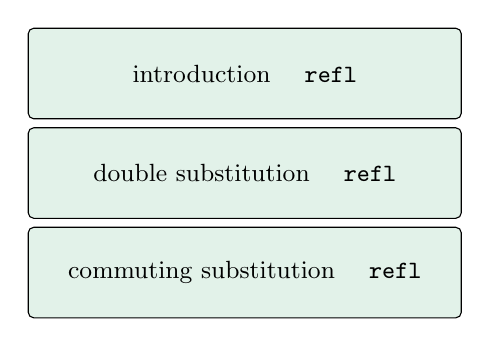
\begin{tikzpicture}[node distance=.1cm]
        \node[system,fill=rorfill,minimum width=5.5cm] (intro) {introduction \quad \refl};
        \node[system,fill=rorfill,minimum width=5.5cm,below=of intro] (double) {double substitution \quad \refl};
        \node[system,fill=rorfill,minimum width=5.5cm,below=of double] (commute) {commuting substitution \quad \refl};
      \end{tikzpicture}
    \end{column}
  \end{columns}

  \vspace{.45em}
  \begin{description}
  \item[Pros:] \textcolor{alu-darkblue}{Inductive syntax, intrinsically typed,
      much gets definitional.}
  \item<2->[Cons:] \textcolor{alu-darkblue}{Not confluent, some benchmarks break.}
  \end{description}
\end{frame}

\begin{frame}{EW: A Roadblock}
      \begin{block}{Desired equation (η-weak)}
        \[
        \bigl(\lambda((N\Wk)\,\Blob)\bigr)\Wk
        \;\equiv\;
        \lambda\bigl(((N\Wk)\Wk)\,\Blob\bigr)
        \]
      \end{block}
      \begin{alertblock}{Both sides are normal forms in Explicit Weakening}
        \centering
        \vspace{.5em}
        \Large
        \(\underbrace{(\lambda\cdots)\Wk}_{\text{outer constructor }\Wk}\)
        \quad vs.\quad
        \(\underbrace{\lambda(\cdots)}_{\text{outer constructor }\lambda}\)
        \vspace{.5em}
      \end{alertblock}
      % \centering
      % \textcolor{alu-red}{No propositional proof can exist.}

  % \begin{columns}[T,onlytextwidth]
  %   \begin{column}{.47\textwidth}
  %     \small
  %     This is weakening commuting with η-expansion, written in the shared notation.
  %   \end{column}
  %   \begin{column}{.47\textwidth}
  %   \end{column}
  % \end{columns}

\end{frame}

\section{Return of the Renamings}

\begin{frame}{Return of the Renamings (RoR)}
  \begin{columns}[c,onlytextwidth]
    \begin{column}{.56\textwidth}
      \begin{block}{Familiar ground}
      \begin{itemize}
        \item Terms are inductive data
        \item Variables are de Bruijn indices
        \item Renamings return as maps
        \item Substitutions are maps
        \item Ren and Sub mostly opaque
        \item Rewriting installs σ-like theory with proved equations
      \end{itemize}
      \end{block}
    \end{column}
    \begin{column}{.39\textwidth}
      \begin{tikzpicture}[node distance=.55cm]
        \node[system,fill=rorfill,minimum width=3.8cm] (terms) {inductive terms};
        \node[system,fill=sigmafill,minimum width=3.8cm,below=of terms] (ren) {first-class renamings};
        \node[system,fill=sigmafill,minimum width=3.8cm,below=of ren] (sub) {substitution interface};
        \draw[implication] (terms) -- (ren);
        \draw[implication] (ren) -- (sub);
      \end{tikzpicture}
    \end{column}
  \end{columns}
\end{frame}

\begin{frame}{RoR: Mapping from EW notation}
      \begin{block}{Presentation notation}
        \[
        \begin{array}{rcl}
          \Blob &\coloneqq& \mathsf{var}\;\mathsf{here}\\
          \lambda N &\coloneqq& \mathsf{lam}\;N\\
          L\,M &\coloneqq& \mathsf{app}\;L\;M\\
          M\Wk &\coloneqq& M[\mathsf{wk}^{R}]^{R}\\
          M[\sigma] &\coloneqq& M[\sigma]^{S}
        \end{array}
        \]
      \end{block}
  % \begin{columns}[T,onlytextwidth]
  %   \begin{column}{.41\textwidth}
  %   \end{column}
  %   \begin{column}{.53\textwidth}
  %     \begin{block}{Extracted from \texttt{STLC70Notation.agda}}
  %       \begingroup
  %         \fontsize{7.1}{8.2}\selectfont
  %         \RoRWeakenByRenaming
  %       \endgroup
  %     \end{block}
  %     \vspace{.5em}
  %     \centering
  %     \textcolor{alu-darkblue}{The aligned syntax is presentation-only; the representation is not.}
  %   \end{column}
  % \end{columns}
\end{frame}

\begin{frame}{RoR: Rewrite theory}
  \begin{columns}[T,onlytextwidth]
    \begin{column}{.37\textwidth}
      \begin{block}{σ-calculus equations (excerpt)}
        \small
        \begin{align*}
          M[\rho]^R[\rho']^R &\rightsquigarrow M[\rho\mathbin{;}\rho']^R\\
          M[\rho]^R[\sigma]^S &\rightsquigarrow M[\langle\rho\rangle\mathbin{;}\sigma]^S\\
          M[\sigma]^S[\tau]^S &\rightsquigarrow M[\sigma\mathbin{;}\tau]^S
        \end{align*}
        % identities, lifting, weakening, and their interactions
      \end{block}
    \end{column}
    \begin{column}{.57\textwidth}
      \begin{block}{Manufacturing definitional equality}
        \small
        \begin{enumerate}
          \item \texttt{opaque} definitions of Ren and Sub
          \item expose \emph{only} equations as rewrite rules
          \item check compatibility with reduction (local confluence)
        \end{enumerate}
      \end{block}
      \begin{alertblock}{On η-id and η-law}
        \begin{itemize}
        \item not rewrite rules
        \item break confluence
        \end{itemize}
      \end{alertblock}
    \end{column}
  \end{columns}

  \note{[Sources] The local STLC70.agda and the ESOP'27 System F development use opaque definitions plus selected rewrite rules; Agda's confluence checker checks the combined reduction and rewrite relation by conservative syntactic criteria.}
\end{frame}

\begin{frame}{RoR: proves what EW cannot}
  \begin{columns}[T,onlytextwidth]
    \begin{column}{.46\textwidth}
      \begin{block}{Return of the Renamings}
        % \begingroup
        % \fontsize{6.8}{7.8}\selectfont
        \small
          \RoRWeakeningEta
        % \endgroup
      \end{block}
      \centering
      \Large\textcolor{alu-green}{\refl}
    \end{column}
    \begin{column}{.48\textwidth}
      \begin{alertblock}{Explicit Weakening}
        \[
        \bigl(\lambda((N\Wk)\,\Blob)\bigr)\Wk
        \not\equiv
        \lambda\bigl(((N\Wk)\Wk)\,\Blob\bigr)
        \]
        \small Outer constructors remain distinct.
      \end{alertblock}
      \centering
      \Large\textcolor{alu-red}{impossible}
    \end{column}
  \end{columns}

  \vspace{.75em}
  % \centering
  % Same surface equation.  The representation changes its computational fate.
\end{frame}

\begin{frame}{Explicit Weakening embeds into RoR}
  \begin{center}
    \begin{tikzpicture}[node distance=2.4cm]
      \node[system,fill=ewfill,minimum width=4.4cm] (ew) {Explicit Weakening\\term / substitution};
      \node[system,fill=rorfill,minimum width=4.4cm,right=of ew] (ror) {Return of the Renamings\\term / substitution};
      \draw[implication] (ew) -- node[above,font=\small,text=alu-darkblue] {translaton} (ror);
    \end{tikzpicture}
  \end{center}

  \vspace{1em}
  \begin{block}{Preservation}
    Translation commutes with instantiation and composition. \\
    $\Rightarrow$ every
    EW-equality is also a RoR-equality.
  \end{block}

  \vspace{.55em}
  \begin{center}
    \Large EW \(\subsetneq\) RoR
    \qquad
    \normalsize strict by η-weak
  \end{center}
\end{frame}

\begin{frame}{RoR vs. σ-calculus; aka the meaning of ``almost''}
  \begin{columns}[T,onlytextwidth]
    \begin{column}{.4\textwidth}
      \begin{block}{η-id}
        \[
          \mathsf{var}\;\mathsf{here} \mathbin{\cdot^S} \mathsf{wk}^S
          \;\equiv\; \mathsf{id}^S
        \]
      \end{block}
      \begin{block}{η-law}
        \vspace{-\baselineskip}
        \[
          \bigl(\mathsf{var}\;\mathsf{here}[\sigma]^S\bigr)
          \mathbin{\cdot^S}
          \bigl(\mathsf{wk}^S\mathbin{;}\sigma\bigr)
          \;\equiv\; \sigma
        \]
      \end{block}
    \end{column}
    \begin{column}{.56\textwidth}
      \begin{itemize}
        \item Both implied by full σ-calculus
        \item Neither is definitional in RoR
        \item Propositional proof ``on top'' of RoR when needed; not just \refl{}
      \end{itemize}
    \end{column}
  \end{columns}

\end{frame}

\section{Evidence and design space}

\begin{frame}{RoR scales}
  \begin{columns}[T,onlytextwidth]
    \begin{column}{.58\textwidth}
  \begin{block}{Formalizing System F}
    \begin{itemize}
    \item Term substitution and type substitution
    \item Terms indexed by types: $Expr\ \Gamma\ T$
    \item $\dots$ which get substituted: $Expr\ \Gamma\ (T[id])$
    \item $\dots$ but $T \not\equiv T[id]$,
    \item $\dots$ so we either insert transports or make $T \equiv T[id]$
      definitional!
    \item $\dots$ transports can leak into lemmas
    \item $\dots$ better make them definitional
    \end{itemize}
  \end{block}
    \end{column}
    \begin{column}{.38\textwidth}
      \begin{block}{Proof of the pudding}
        Transports disappear in proofs
        \begin{itemize}
        \item canonicity for System F
        \item logical relations
        % \item all POPLmark challenge parts for System F\\
        %   (intrisically scoped; Autosubst)
        \end{itemize}
      \end{block}
    \end{column}
  \end{columns}
  % why is System F interesting!

  % \begin{columns}[c,onlytextwidth]
  %   \begin{column}{.56\textwidth}
  %     \small
  %   \end{column}
  %   \begin{column}{.38\textwidth}
  %     \begin{tikzpicture}[node distance=.32cm]
  %       \node[system,fill=sigmafill,minimum width=3.8cm,minimum height=.9cm] (canon) {canonicity};
  %       \node[system,fill=sigmafill,minimum width=3.8cm,minimum height=.9cm,below=of canon] (lr) {logical relation};
  %       \node[system,fill=sigmafill,minimum width=3.8cm,minimum height=.9cm,below=of lr] (popl) {POPLmark};
  %     \end{tikzpicture}
  %   \end{column}
  % \end{columns}

  % \vspace{.25em}
  % \begin{center}
  %   \small
  %   \textcolor{alu-darkblue}{\textbf{What remains explicit:}}
  %   the semantic argument and the interesting induction.\\
  %   Administrative substitution transports disappear into normalization.
  % \end{center}

  \note{[Sources] Local ESOP'27 Agda development, including SystemF.agda and SystemF-strat.agda; the latter contains SN-all and canonicity.}
\end{frame}

\begin{frame}{Overview}
  \footnotesize
  \renewcommand{\arraystretch}{1.25}
  \setlength{\tabcolsep}{3pt}
  \begin{tabular}{>{\bfseries}p{.12\textwidth} p{.1\textwidth} p{.27\textwidth}
    p{.24\textwidth} p{.1\textwidth}}
    \toprule
    & Inductive terms & Variables & Equational strength & Confluence\\
    \midrule
    σ-calculus
      & \no{}
      & unified term/substitution calculus
      & full theory, including η
    & \yes\\
    RoR
      & \yes
      & de Bruijn + renamings
      & extended σ-laws; no η 
    & \yes\\
    EW
      & \yes
      & \(\Blob\) + explicit \(\_\Wk\) constructor
      & weaker again
    & \no \\
    \bottomrule
  \end{tabular}

  \vspace{1.0em}
  \begin{center}
    \begin{tikzpicture}[node distance=1.2cm]
      \node[system,fill=sigmafill,minimum width=3.1cm] (sigma) {σ-calculus};
      \node[system,fill=rorfill,minimum width=3.7cm,right=of sigma] (ror) {Return of the\\Renamings};
      \node[system,fill=ewfill,minimum width=3.3cm,right=of ror] (ew) {Explicit\\Weakening};
      \draw[-{Stealth[length=2.5mm]},line width=1.1pt] (ew) -- node[above,font=\small] {strict} (ror);
      \draw[-{Stealth[length=2.5mm]},line width=1.1pt] (ror) -- node[above,font=\small] {strict} (sigma);
    \end{tikzpicture}
  \end{center}
\end{frame}

\begin{frame}{All you need is \refl{} --- almost}
      \begin{enumerate}
        \item σ-calculus: full equational theory
        \item EW regains inductive syntax,
          but rules out useful equalities, \\
          confluence?\footnote{Non-confluent rewrite rules make definitional equality depend on the reduction path, undermining predictable type checking.}
        \item RoR keeps inductive syntax and standard variables while recovering
          a strictly stronger, confluent theory \\
          demonstrated to work on significant developments
      \end{enumerate}

  % \vspace{.7em}
  % \begin{center}
  %   \Large Choose the representation so that bureaucracy computes---\\[.2em]
  %   \textcolor{alu-darkblue}{and save proofs for the mathematics.}
  % \end{center}
\end{frame}



\begin{frame}{Questions?}
  \begin{center}
    \vspace{.8em}
    \Huge All You Need Is \refl

    \vspace{.35em}
    \Large --- Almost

    \vspace{1.5em}
    \normalsize
    Peter Thiemann \quad Marius Weidner
  \end{center}
\end{frame}

\appendix
\section{Backup}

\begin{frame}{Backup: benchmark equations}
  \scriptsize
  \renewcommand{\arraystretch}{1.45}
  \setlength{\tabcolsep}{4pt}
  \begin{tabular}{>{\bfseries}p{.32\textwidth} p{.62\textwidth}}
    Introduction & \((N\Wk)[M]_0 \equiv N\) \\
    Double substitution & \(N[M]_1[L]_0 \equiv N[L\Wk]_0[M]_0\) \\
    Commuting substitution & \(N[M]_0[L]_0 \equiv N[L]_1[M[L]_0]_0\) \\
    Through η-expansion & \((\lambda(N\Wk\,\Blob))[\sigma] \equiv \lambda((N[\sigma])\Wk\,\Blob)\) \\
    Through single substitution & \((N[\mathsf{id}\mathbin{\rhd}M])[\sigma]
      \equiv (N[\sigma\Wk\mathbin{\rhd}\Blob])[\mathsf{id}\mathbin{\rhd}(M[\sigma])]\) \\
    Weakening through η & \((\lambda(N\Wk\,\Blob))\Wk \equiv \lambda((N\Wk)\Wk\,\Blob)\) \\
    η-id & \((\mathsf{id}\Wk)\mathbin{\rhd}\Blob \equiv \mathsf{id}\) \\
    η-law & \(((\mathsf{id}\Wk)\mathbin{;}\sigma)\mathbin{\rhd}(\Blob[\sigma]) \equiv \sigma\) \\
  \end{tabular}
\end{frame}

\begin{frame}{Backup: typed pieces behind the notation}
  \small
  \begin{columns}[T,onlytextwidth]
    \begin{column}{.47\textwidth}
      \begin{block}{Explicit Weakening}
        \[
        \begin{array}{ll}
          \Blob &: \Gamma\rhd A \vdash A\\
          \_\Wk &: \Gamma\vdash A \to \Gamma\rhd B\vdash A\\
          \mathsf{id} &: \Gamma\models\Gamma\\
          \_\Wk &: \Gamma\models\Delta \to \Gamma\rhd A\models\Delta\\
          \_\rhd\_ &: \Gamma\models\Delta \to \Gamma\vdash A
            \to \Gamma\models\Delta\rhd A
        \end{array}
        \]
      \end{block}
    \end{column}
    \begin{column}{.47\textwidth}
      \begin{block}{Return of the Renamings}
        \[
        \begin{array}{ll}
          \mathsf{here} &: \Gamma\rhd A \ni A\\
          \mathsf{there} &: \Gamma\ni A \to \Gamma\rhd B\ni A\\
          \mathsf{var} &: \Gamma\ni A \to \Gamma\vdash A\\
          \mathsf{Ren}\;\Delta\;\Gamma &: \Delta\ni A \to \Gamma\ni A\\
          \mathsf{Sub}\;\Delta\;\Gamma &: \Delta\ni A \to \Gamma\vdash A
        \end{array}
        \]
      \end{block}
    \end{column}
  \end{columns}

  \vspace{.5em}
  \centering
  Both substitution notations read \(M:\Delta\vdash A\) and
  \(\sigma:\Delta\to\Gamma\),
  hence \(M[\sigma]:\Gamma\vdash A\).
\end{frame}

% \begin{frame}{Backup: the strictness witness is machine-checked}
%   \begin{columns}[T,onlytextwidth]
%     \begin{column}{.47\textwidth}
%       \begin{block}{RoR: extracted proof}
%         \begingroup
%           \fontsize{6.6}{7.5}\selectfont
%           \RoRWeakeningEta
%         \endgroup
%       \end{block}
%     \end{column}
%     \begin{column}{.47\textwidth}
%       \begin{alertblock}{EW: extracted impossibility proof}
%         \small
%         \[
%           \bigl((\lambda((N\Wk)\Blob))\Wk
%           \equiv \lambda(((N\Wk)\Wk)\Blob)\bigr) \to \bot
%         \]
%         \begingroup
%           \footnotesize
%           \EWComparisonWeakeningEtaImpossibleProof
%         \endgroup
%       \end{alertblock}
%     \end{column}
%   \end{columns}
% \end{frame}

% \begin{frame}{Backup: the full σ-calculus reaches η}
%   \begin{columns}[T,onlytextwidth]
%     \begin{column}{.47\textwidth}
%       \begin{block}{η-id}
%         \small
%         \[
%           \mathsf{var}\;\mathsf{here} \mathbin{\cdot^S} \mathsf{wk}^S
%           \equiv \mathsf{id}^S
%         \]
%         \begingroup
%           \footnotesize
%           \LSEtaIdProof
%         \endgroup
%       \end{block}
%     \end{column}
%     \begin{column}{.47\textwidth}
%       \begin{block}{η-law}
%         \small
%         \[
%           (\mathsf{var}\;\mathsf{here}[\sigma]^S)
%           \mathbin{\cdot^S}(\mathsf{wk}^S\mathbin{;}\sigma)
%           \equiv \sigma
%         \]
%         \begingroup
%           \footnotesize
%           \LSEtaLawProof
%         \endgroup
%       \end{block}
%     \end{column}
%   \end{columns}
% \end{frame}

\end{document}
